\documentclass[tikz,border=5mm]{standalone}
\begin{document}
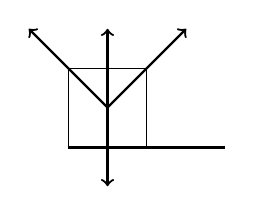
\begin{tikzpicture}
    % Draw the box
    \node[rectangle,draw,minimum size=1cm](box){};
    
    % Draw the forces
    \draw[->,thick](box.center)--++(0,-1) node[midway,right]{}; % Gravity
    \draw[->,thick](box.center)--++(0,1) node[midway,right]{}; % Normal
    \draw[->,thick](box.center)--++(-1,1) node[midway,above]{}; % Applied force 1
    \draw[->,thick](box.center)--++(1,1) node[midway,above]{}; % Applied force 2
    
    % Draw the ground
    \draw[thick] (box.south west)--++(2,0);
    \end{tikzpicture}
\end{document}